\documentclass[12pt]{article}
\usepackage[usenames, dvipsnames, table]{xcolor}
\usepackage[utf8]{inputenc}
\usepackage{amsmath}
\usepackage{amsfonts}
\usepackage{comment}
\usepackage{wrapfig}
\usepackage{booktabs}
\usepackage{tikz}
\usepackage{gnuplottex}
\usepackage{epstopdf}
\usepackage{marginnote}
\usepackage{float}
\usetikzlibrary{tikzmark}
\usepackage{graphicx}
\usepackage{cancel}
\usepackage{bm}

\usepackage{hyperref}

\newif\ifquoteopen
\catcode`\"=\active % lets you define `"` as a macro
\DeclareRobustCommand*{"}{%
   \ifquoteopen
     \quoteopenfalse ''%
   \else
     \quoteopentrue ``%
   \fi
}

\PassOptionsToPackage{table}{xcolor}

\usepackage{soul}

\newcommand{\hlc}[2]{%
  \colorbox{#1!50}{$\displaystyle#2$}}


\usepackage[a4paper,
            total={170mm,257mm},
 left=20mm,
 top=20mm]{geometry}

\newcommand{\q}[1]{``#1''}
\newcommand{\lamb}[2]{\Lambda^{#1}_{\>{#2}}}
\usepackage{fancyhdr}
\pagestyle{fancy}
\fancyhead{} % clear all header fields
\renewcommand{\headrulewidth}{0pt} % no line in header area
\fancyfoot{} % clear all footer fields
\fancyfoot[LE,RO]{\thepage}           % page number in "outer" position of footer line
\fancyfoot[RE,LO]{Francesco Manzali, Marzo 2018} % other info in "inner" position of footer line

\begin{document}
\section{Elettromagnetismo, principio di relatività e trasformazioni di Galileo}
Con lo studio dell'elettromagnetismo sorge spontanea una domanda: le equazioni di Maxwell rispettano il principio di relatività? Assumono cioè la stessa forma in tutti i sistemi di riferimento inerziali?\\
Con qualche conto si scopre che, se usiamo le trasformazioni di Galileo per il passaggio da un sdr inerziale ad un altro, allora le equazioni di Maxwell \textbf{non} sono covarianti. Dimostriamolo.\\
Si consideri un sdr cartesiano $S$ inerziale in cui si ha una particella carica $q$ in moto rettilineo con velocità iniziale $\vec{v}=v\hat{x}$, soggetta all'azione di un campo magnetico $\vec{B} = B(x,t)\hat{z}$ ed elettrico $\vec{E} = E(x,t)\hat{y}$.\\
La particella subisce una forza data da $\vec{F} = q(\vec{E}+\vec{v}\times\vec{B}) = q(E-vB)\hat{y}$. Poiché $\vec{B}$ ha componenti solo lungo $\hat{z}$ il suo rotore è dato da:
\[
\vec{\nabla}\times\vec{B} = \operatorname{det}\begin{bmatrix}
\hat{x} & \hat{y} & \hat{z}\\
\frac{\partial}{\partial x} & \frac{\partial}{\partial y} & \frac{\partial}{\partial z}\\
0 & 0 & B(x,t)
\end{bmatrix}
= \frac{\partial B}{\partial y}\hat{x}-\frac{\partial B}{\partial t}\hat{y}
\]
dove si è usato il fatto che $B$ considerato dipende solo da $x$. Applicando la quarta equazione di Maxwell (nel vuoto) si ottiene perciò: $\vec{\nabla}\times\vec{B} = -\frac{\partial B}{\partial x}\hat{y} = \frac{1}{c^2}\frac{\partial \vec{E}}{\partial t} = \frac{\partial E}{\partial t}\hat{y}$, e proiettando su $\hat{y}$ si giunge a:
\[
\frac{\partial B}{\partial x} = -\frac{1}{c^2}\frac{\partial E}{\partial t}
\]
Si consideri ora un altro sdr cartesiano $S'$ in moto rettilineo uniforme con velocità $V\hat{x}$ rispetto ad $S$, nel quale i campi misurano $B'$ e $E'$ (e mantengono la stessa direzione, per evitare di originare nelle equazioni di Maxwell termini nuovi che modificano la direzione della forza risultante).\\
Le trasformazioni di Galileo sono:
\[
\begin{cases}
x' = x-Vt\\
t' = t
\end{cases}
\]
$S'$ è inerziale, per cui l'accelerazione subita dalla carica non cambia, e perciò la forza risultante su di essa deve essere la stessa che era presente in $S$. Proiettando lungo $\hat{y}$ si ottengono le trasformazioni per i campi:
\[
q(E-vB) = q(E'-v'B) = q(E'-vB')+VB' \Rightarrow \begin{cases}E = E' + VB'\\B = B' \end{cases} 
\]
dove $v'$ è la velocità di $q$ in $S'$, e si ha $v' = v-V$ per trasformazioni di Galileo.\\
Per \emph{principio di relatività} le leggi della fisica sono le \textbf{stesse} in tutti i sistemi di riferimento inerziali e in particolare per $S'$. Perciò se in $S$ vale:
\[
\frac{\partial B}{\partial x} = -\frac{1}{c^2}\frac{\partial E}{\partial t}
\]
ci si aspetta che in $S'$ valga l'analogo:
\[
\frac{\partial B'}{\partial x'} = -\frac{1}{c^2}\frac{\partial E'}{\partial t'}
\]
Derivando le trasformazioni dei campi si ottiene:
\begin{equation}
\frac{\partial E}{\partial t} = \frac{\partial E'}{\partial t} + V\frac{\partial B'}{\partial t};\quad \frac{\partial B}{\partial x} = \frac{\partial B'}{\partial x}
\end{equation}
$E'$ e $B'$ sono funzioni di $x'$ e $t'$, ciascuno dei quali è funzione a sua volta di $x$ e $t$. Applicando la regola della catena si possono calcolare le derivate comparse:
\begin{align*}
    \frac{\partial E'}{\partial t} &= \frac{\partial E'}{\partial x'}\underbrace{\frac{\partial x'}{\partial t}}_{-V} + \frac{\partial E'}{\partial t'}\underbrace{\frac{\partial t'}{\partial t}}_{1} = -v\frac{\partial E'}{\partial x'} + \frac{\partial E'}{\partial t'}\\
    \frac{\partial B'}{\partial x} &= \frac{\partial B'}{\partial x'}\underbrace{\frac{\partial x'}{\partial x}}_{1}+\frac{\partial B'}{\partial t'}\underbrace{\frac{\partial t'}{\partial x}}_{0} = \frac{\partial B'}{\partial x'}\\
    \frac{\partial B'}{\partial t} &= \frac{\partial B'}{\partial x'}\underbrace{\frac{\partial x'}{\partial t}}_{-V}+\frac{\partial B'}{\partial t'}\underbrace{\frac{\partial t'}{\partial t}}_{1} = -V\frac{\partial B'}{\partial x'}+\frac{\partial B'}{\partial t'}
\end{align*}
in cui si sono già sostituite le derivate ottenute dalle trasformazioni di Galileo:
\begin{align*}
    \frac{\partial x'}{\partial x} = 1 & & \frac{\partial x'}{\partial t} &= -V\\
    \frac{\partial t'}{\partial t} = 1 & & \frac{\partial t'}{\partial x} &= 0
\end{align*}
Sostituendo quindi nelle derivate delle trasformazioni dei campi: %Inserire ref
\begin{align*}
\frac{\partial E}{\partial t} &= -V\frac{\partial E'}{\partial x'}+\frac{\partial E'}{\partial t'}-V^2\frac{\partial B'}{\partial x'}+V\frac{\partial B'}{\partial t'}\\
\frac{\partial B}{\partial x} &= \frac{\partial B'}{\partial x'}
\end{align*}
E infine sostituendo nell'espressione ricavata dalle leggi di Maxwell:
\[
\frac{\partial B}{\partial x}=-\frac{1}{c^2}\frac{\partial E}{\partial t}\Rightarrow \frac{\partial B'}{\partial x'} = -\frac{1}{c^2}\frac{\partial E'}{\partial t'}+\frac{V}{c^2}\underbrace{\left ( \frac{\partial E'}{\partial x'} + V\frac{\partial B'}{\partial x'} - \frac{\partial B'}{\partial t'}\right )}_{\neq 0}
\]
La presenza di un termine in più generalmente non nullo fa sì che le equazioni di Maxwell non siano invarianti rispetto alle trasformazioni di Galileo.\\
\subsection{Conseguenze}
Il risultato appena ricavato ci lascia, essenzialmente, tre possibilità.
\begin{enumerate}
    \item \textbf{Principio di relatività solo per la meccanica}. Magari quanto abbiamo calcolato è tutto giusto, per cui dobbiamo dire che \textit{le equazioni di Maxwell assumono la loro forma usuale in un sistema di riferimento "speciale"}, che viene chiamato \textbf{etere}.
    Così, stando in un sistema di riferimento solidale all'etere valgono tutte le conseguenze delle equazioni di Maxwell: per esempio un tale osservatore misura come velocità di propagazione della luce esattamente $c$.\\
    Tuttavia, un osservatore che \textit{si muove} rispetto all'etere osserverà - per trasformazioni di Galileo - una velocità di propagazione della luce \textit{diversa} ($c \pm v$, con $v$ la velocità relativa dei sdr). Questa conseguenza \textit{può} essere investigata sperimentalmente.
    \item \textbf{Principio di relatività per meccanica ed elettromagnetismo}. Tuttavia l'esistenza di un sistema di riferimento speciale è, tutto sommato, una scocciatura. Sarebbe bello se il \textit{principio di relatività} valesse \textit{per tutta la fisica}. Tuttavia, come abbiamo notato, le equazioni di Maxwell non rispettano tale principio se usiamo le trasformazioni di Galileo. Trascurando l'ipotesi terribile che tutto sia sbagliato, abbiamo due possibilità:
    \begin{enumerate}
        \item \textbf{Modifica  relativistica delle equazioni di Maxwell}. Potrebbero essere giuste le trasformazioni di Galileo, e sbagliate le equazioni di Maxwell. Sperimentalmente dovremmo perciò osservare delle situazioni in cui \textit{non valgono} le leggi di Maxwell, e partire da esse per modificare l'elettromagnetismo rendendolo compatibile con le trasformazioni galileiane e covariante.
        \item \textbf{Modifica relativistica delle trasformazioni di Galileo}. Questa è l'ipotesi peggiore, poiché se c'è un errore nelle trasformazioni di Galileo significa che anche la meccanica classica newtoniana, che va di pari passo con esse, è da rivedere. Anche qui dovremmo comunque essere in grado di notare \textit{problemi} a livello sperimentale. 
    \end{enumerate}
\end{enumerate}


\section{Esperimenti sulla velocità della luce}
Sperimentalmente si osserva tuttavia che la velocità della luce è effettivamente la stessa \textit{rispetto a qualsiasi sistema di riferimento}. Tali risultati, raffinati nel corso di diversi anni, porteranno poi alla necessità di una nuova meccanica.

\subsection{Le lune di Io}
La prima misura della velocità della luce fu fatta nel 1676 dall'astronomo danese Ole Rømer. In figura \ref{fig:rivoluzioni-io} è disponibile uno schema dell'esperimento.\\
\begin{wrapfigure}{r}{0.3\textwidth}
\begin{center}
    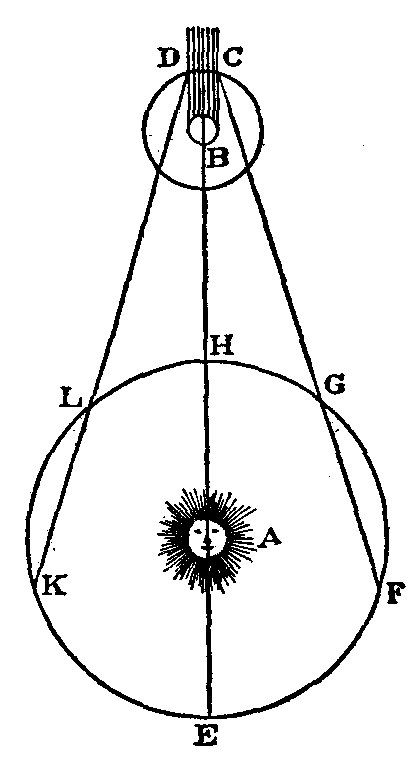
\includegraphics[width=0.28\textwidth]{Grafica/IoRevolutions.png}
\end{center}
\caption{Rivoluzioni di Io}
\label{fig:rivoluzioni-io}
\end{wrapfigure}
Ogni $42$ ore e mezzo, il satellite di Giove (in $B$) Io entra nell'ombra del pianeta, e scompare dalla vista degli astronomi. A seconda della posizione del periodo dell'anno (e quindi della posizione della Terra rispetto a quella di Giove) è possibile osservare l'entrata ($C$) di Io nell'ombra di Giove (se la Terra si trova in $G$ o in $F$) oppure l'uscita ($D$) (se la Terra si trova in $L$ o $K$) oppure nessuna delle due (quando la Terra è in $E$, le eclissi avvengono di giorno). Misurando il tempo che intercorre tra un passaggio e l'altro si ottiene una stima del periodo orbitale di Io.\\
Poiché la velocità della luce è finita, tale misura \textit{cambia} a seconda che la Terra si stia avvicinando o allontanando da Giove. Se la Terra passa da $F$ a $G$ (avvicinandosi), allora il segnale della prima eclissi arriva all'occhio dell'osservatore con un ritardo pari a $t_F$, necessario a percorrere la distanza $CF$, ma all'eclissi successiva, che avviene dopo un tempo $T$, la Terra si trova in $G$ (lo spostamento non è in scala) e quindi il segnale impiegherà un $t_G < t_F$ per arrivare, poiché la distanza $CG$ è minore di $CF$ (la Terra si è avvicinata). L'astronomo misurerà perciò un periodo diverso da quello reale:
\[
T'_{\text{avv}} = (T+t_G)-t_F = T + \frac{d_G - d_F}{c} < T; \quad d_G < d_F
\]
D'altro canto, se la Terra si sta allontanando, per esempio passando da $L$ a $K$, allora il ritardo aumenta alla seconda osservazione:
\[
T'_{\text{all}} = (T+t_K)-t_L = T + \frac{d_K-d_L}{c} > T; \quad d_K > d_L
\]
Se le misurazioni avvengono simmetricamente, ossia se $d_G$ = $d_L$ e $d_F$ = $d_K$, allora si avrà $|d_G-d_F|=|d_F-d_K|=\Delta d$, e $T'_{\text{avv}} = T-\Delta d/c$, $T'_{\text{all}} = T+\Delta d/c$. Sottraendo membro a membro si ottiene:
\[
\Delta T' = T'_{\text{all}}-T'_{\text{acc}} = \frac{2\Delta d}{c}
\]
La massima $\Delta d$ disponibile è pari al diametro della circonferenza terrestre (corrisponderebbe a prendere le misure tra $E$ e $H$), ed è praticamente infattibile, in quanto in tali punti non è possibile osservare le eclissi di Io. Per ottenere una stima di ordini di grandezza, tuttavia, poniamo $\Delta d = 2R$, da cui $\Delta T' = 4R/c$.\\
Finora abbiamo ipotizzato che la velocità della luce sia costante, ma è necessario verificarlo. Diciamo che esiste un sistema di riferimento, detto \textit{etere}, rispetto al quale la luce si muove in $c$. Se il sistema solare si muove rispetto all'etere a velocità $v$, allora la velocità della luce osservata varia a seconda che il segnale si muova nello stesso senso, o in senso opposto, al moto del sistema solare.\\
Ipotizziamo, per esempio, che il sistema raffigurato in (\ref{fig:rivoluzioni-io}) si muova verso l'alto a velocità $v$. Allora, se effettuiamo le misure di sopra quando Giove è nella posizione indicata, i segnali delle eclissi di Io saranno diretti in verso \textit{opposto} al movimento del sistema, e perciò si propagheranno, rispetto alla Terra, a $c+v$. Se invece Giove si trovasse in basso (sotto a $E$) %Fare bene figura, magari
allora il segnale sarebbe emesso nello stesso verso del moto, e quindi da Terra si osserverebbe una velocità $c-v$. Tali variazioni comportano due misurazioni differenti dei tempi:
\[
\Delta T'_1 = \frac{4R}{c+v}; \quad \Delta T'_2 = \frac{4R}{c-v} 
\]
la cui differenza è data da:
\[
\delta t = \Delta T'_1 - \Delta T'_2 = \frac{4R}{(c+v)(c-v)}(c+v-c+v) = \frac{8Rv}{c^2-v^2} = \frac{8Rv}{c^2\displaystyle \left(1-\frac{v^2}{c^2} \right )}
\]
%Ricavare v esplicitamente
Per cui un $\delta t = 1$s corrisponde a $v = 150$km/h. Sperimentalmente non viene osservata alcuna $\delta t$, ma le misure non sono sufficientemente precise per dare certezza (date anche le enormi difficoltà per metterle in pratica).\\
Alternativamente, potrebbe essere che il sistema di riferimento dell'etere sia solidale a quello del sistema solare.

\subsection{Esperimento di Michelson e Morley}
%Inserire immagine
Nel caso di etere stazionario\footnote{Nel senso di non "trascinato" da corpi in movimento} e solidale al sistema solare, è possibile misurare alcune differenze nei tempi di percorrenza della luce in diverse direzioni, giungendo a una stima della velocità di rivoluzione della Terra attorno al Sole (che si sa essere dell'ordine di $30$km/s).\\
Nel 1887 i fisici Michelson e Morley effettuarono un esperimento per determinare ciò.\\
Un raggio di luce viene fatto passare attraverso uno specchio semiargentato posto all'origine di un sistema di riferimento cartesiano a $t=0$, in modo che uno dei fasci risultanti sia emesso lungo $\hat{x}$, che immaginiamo (per semplicità) essere nella stessa direzione del moto attraverso l'etere\footnote{Chiaramente tale direzione non è conoscibile a priori, e perciò l'esperimento è stato ripetuto in diverse orientazioni, e a diversi periodi dell'anno - poiché in principio potrebbe succedere che ci siano giorni in cui la Terra è solidale all'etere.}, e l'altro lungo l'asse $y$ (fascio trasverso). I due fasci vengono fatti riflettere su due specchi, posti a distanze $L_1$ e $L_2$ dall'origine. Al ritorno, i due segnali si ricongiungono allo specchio semiargentato, e una parte della loro sovrapposizione è riflessa verso uno schermo.\\
Esaminiamo ciò che succede dal punto di vista di un osservatore solidale all'etere.\\
Il fascio lungo l'asse $x$ lascia l'origine a $t=0$ e raggiunge lo specchio al tempo $t_1$, muovendosi a $c$. Nel frattempo, lo specchio, inizialmente posto a distanza $L_1$ dall'origine, si è spostato di un ulteriore $vt_1$, e perciò:
\[
c t_1 = L+v t_1 \Rightarrow t_1 = \frac{L_1}{c-v}
\]
Durante il viaggio di ritorno il calcolo è lo stesso, ma col segno di $v$ invertito (ora è lo specchio semiargentato che \textit{si avvicina} al fascio in arrivo). Sia $t_2$ il tempo impiegato dal raggio a tornare all'origine:
\[
c t_2 = L-v t_2 \Rightarrow t_2 = \frac{L_1}{c+v}
\]
Il tempo totale di percorrenza è quindi:
\[
T_{dir.} = t_1+t_2 = \frac{L_1}{c-v} + \frac{L_1}{c+v} = \frac{2L_1}{c\left ( 1- \frac{v^2}{c^2}\right )}
\]
Consideriamo ora il fascio trasverso, e sia $t_3$ il tempo necessario perché raggiunga lo specchio, posto a distanza $L_2$ dall'origine. Nel frattempo quest'ultimo si è mosso di $vt_3$ in direzione $x$, perciò la distanza totale percorsa dal raggio è, per Pitagora:
\[
d = \sqrt{L_2^2 + (vt_3)^2} = ct_3 \Rightarrow t_3 = \frac{L_2}{\sqrt{c^2-v^2}}
\]
Per simmetria la distanza è la stessa anche nel cammino di ritorno. Il tempo totale di percorrenza sarà perciò:
\[
T_{trasv.} = 2t_3 = \frac{2L_2}{\sqrt{c^2-v^2}} = \frac{2L_2}{c\sqrt{1-\frac{v^2}{c^2}}}
\]
Perciò i due fasci ritornano all'origine in momenti diversi, con una differenza temporale di:
\[
\Delta t = T_{trasv.} - T_{dir.} = \frac{2}{c}\left [\frac{L_2}{\sqrt{1-\frac{v^2}{c^2}}} - \frac{L_1}{1-\frac{v^2}{c^2}} \right ]
\]
Ruotando il setup di $90^\circ$ e ripetendo i conti con gli assi scambiati si ottiene:
\[
\Delta t' = T_{trasv.}' - T_{dir.}' = \frac{2}{c}\left [ \frac{L_2}{1-\frac{v^2}{c^2}} - \frac{L_1}{\sqrt{1-\frac{v^2}{c^2}}} \right ]
\]
E la differenza tra le due misure è pari a:
\begin{align*}
\Delta t' - \Delta t &= \frac{2}{c}\left [\frac{L_1+L_2}{1-\frac{v^2}{c^2}} - \frac{L_1+L_2}{\sqrt{1-\frac{v^2}{c^2}}} \right ] = \frac{2(L_1+L_2)}{c}\left [ \frac{1}{1-\frac{v^2}{c^2}} - \frac{1}{\sqrt{1-\frac{v^2}{c^2}}} \right ]\\
&\approx \frac{2(L_1+L_2)}{c}\left [ \left (1+\frac{v^2}{c^2}\right ) - \left ( 1+\frac{1}{2}\frac{v^2}{c^2} \right )\right ] = \frac{L_1+L_2}{c}\frac{v^2}{c^2}
\end{align*}
dove si sono usate le espansioni $1/(1-t) = 1 + t + o(t^3)$ e $1/\sqrt{1-t^2} = 1+t^2/2 + o(t^3)$.\\
Tale differenza corrisponde ad una differenza di percorso di $\Delta \lambda = c\Delta T$, che conduce ad uno sfasamento di $\Delta Na$ frange:
\[
\Delta N = \frac{\Delta \lambda}{\lambda} = \frac{c\Delta T}{\lambda} = \frac{L_1+L_2}{\lambda}\frac{v^2}{c^2}
\]
Michelson e Morley usarono un setup con $L_1+L_2 = 11$m, $\lambda = 550$nm, che per $v\approx 30$km/s (moto orbitale della Terra) genera $\Delta N = 0.4$. Sperimentalmente si osserva uno spostamento medio di $0.01$ frange, compatibile con la situazione di nessun spostamento.\\
È tuttavia possibile che l'etere venga "trascinato" dal moto degli oggetti: ciò spiegherebbe il risultato nullo dell'esperimento di Michelson-Morley, in quanto l'etere sarebbe solidale al laboratorio. Tale ipotesi è detta di \textbf{completo trascinamento} dell'etere: tutta la materia che è solidale alla Terra \textit{trascina} con sé l'etere alla stessa velocità. 

\subsection{Aberrazione stellare}
L'ipotesi del trascinamento dell'etere è tuttavia incompatibile con l'osservazione dell'aberrazione stellare.\\ %[TO DO] Immagine
Si consideri una sorgente di luce posta allo zenith, vista da un osservatore in moto a velocità $v$, con $v \ll c$. Per composizione delle velocità (classica), la stella apparirà ad un angolo $\alpha$ con la verticale dato da $\tan\alpha = v/c \approx \alpha$. Nel caso del moto della Terra attorno al sole, $v \approx 30$km/s, da cui $\alpha \sim 10^{-4}$rad.\\
Ripetendo l'esempio dopo $6$ mesi, la velocità della Terra sarà ora opposta, e quindi vi sarà una deviazione di $-\alpha$ dalla verticale. Nel corso dell'anno, perciò, la posizione della stella apparirà muoversi lungo un ellisse attorno allo zenith, con semiassi che dipendono dalle velocità relative dei due corpi celesti.\\
Se ipotizziamo però che l'etere sia trascinato dal moto della Terra, allora ciò non ha senso: l'etere "trascinato" dalla Terra trascinerebbe con sé anche i raggi di luce provenienti dalla stella, che quindi apparirebbero all'osservatore senza alcuna deviazione. Un'animazione esplicativa è disponibile qui: \url{https://goo.gl/6Co3oh}.\\

\subsection{Esperimento di Airy}
\begin{wrapfigure}{r}{0.4\textwidth}
\begin{center}
    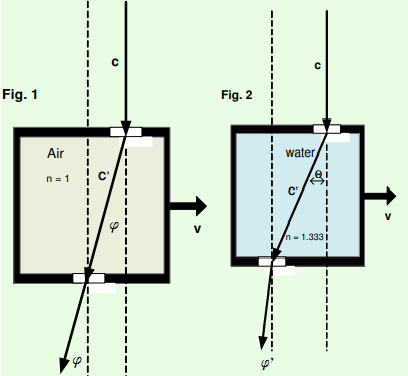
\includegraphics[width=0.38\textwidth]{Grafica/airy.png}
    \caption{Esperimento di Airy, da \url{https://goo.gl/TTfNFf}}
    \label{fig:airy}
\end{center}
\end{wrapfigure}
Il fenomeno dell'aberrazione stellare non è compatibile neanche con l'etere stazionario, come dimostra l'esperimento compiuto nel 1871 da Airy.\\
In una scatola quadrata viene praticato un foro, in cui entra un raggio parallelo alla verticale. Dopo un tempo $\Delta t$, la luce raggiunge il lato opposto della scatola. Se il quadrato non si muove lungo $\hat{x}$ allora il raggio raggiunge il fondo nella posizione subito al di sotto dell'apertura. Se invece la scatola si muove a velocità $v$ lungo $\hat{x}$, allora durante quel $\Delta t$ si sposta a destra di $v\Delta t$, e il raggio - che prosegue muovendosi in verticale - arriverà al fondo in una posizione di $v\Delta t$ più a sinistra di quella a cui sarebbe atterrato se il sistema non si fosse mosso. Ad un osservatore solidale alla scatola il raggio apparirà quindi non più verticale, ma con un angolo $\varphi = \arctan v/c$ rispetto alla verticale stessa.\\
Questo è, in sintesi, l'usuale effetto di aberrazione stellare, in cui l'etere è completamente stazionario, ossia non viene "trascinato" dalla scatola nel suo movimento.\\
Riempiendo la scatola d'acqua, a causa del differente indice di rifrazione la luce impiegherà un tempo $\Delta t' > \Delta t$ per raggiungere il fondo del quadrato. Ci si aspetta quindi che lo spostamento rilevato a sinistra sia maggiore, in quanto in $\Delta t'$ il sistema compirà uno spostamento maggiore. Bisogna però tener conto che l'osservatore, solidale alla scatola, non osserva il raggio in acqua: bisogna quindi calcolare l'angolo di rifrazione all'uscita dal quadrato.\\
Notiamo che il raggio in entrata è perpendicolare alla superficie dell'acqua, e quindi non viene rifratto, ma rallenta ad una velocità $c' = c/n$. L'angolo di aberrazione $\theta$ dovuto allo spostamento del sistema si calcola con la stessa formula di prima, e sarà perciò:
\[
\theta = \arctan \frac{v}{c'} = \arctan v\frac{n}{c} \approx v\frac{n}{c}
\]
dove nell'ultimo passaggio si è adottata l'approssimazione per angoli piccoli. A questo punto il raggio subisce una rifrazione, ed esce ad un angolo $\varphi'$. Applicando la legge di Snell:
\[
n\sin\theta = \sin\varphi' \Rightarrow \sin\varphi' \approx \varphi' \approx v\frac{n^2}{c}
\]
(in quanto l'aria ha un indice di rifrazione $\approx 1$). La differenza con l'angolo misurato con la scatola senz'acqua è quindi:
\[
\varphi'-\varphi = \frac{v}{c}(n^2-1)
\]
Airy effettuò un tale esperimento nel 1871, riempiendo un telescopio d'acqua e cercando di determinare eventuali variazioni nell'angolo di aberrazione, senza però osservarne alcuna. Ciò significa che l'ipotesi dell'etere completamente stazionario è inesatta, e anche quella dell'etere completamente trascinato (o non si osserverebbe alcuna aberrazione).

\subsection{L'esperimento di Fizeau}
Un'idea che potrebbe spiegare l'esperimento di Airy è quella del \textbf{trascinamento parziale} dell'etere, elaborata da Fresnel. L'idea è che l'etere venga trascinato dalla materia, ma solo nel caso essa abbia un indice di rifrazione significativo. Quantitativamente, da argomenti elettromagnetici Fresnel trovò che la velocità della luce in un dielettrico in moto a velocità $v$ è data da:
\[
c' = \frac{c}{n} + v\left ( 1- \frac{1}{n^2}\right )
\]
Poiché l'aria ha indice di rifrazione $\approx 1$ essa non provoca alcun trascinamento, e quindi l'aberrazione stellare risulta visibile. D'altro canto l'acqua, con $n = 1.33$, trascina parzialmente l'etere, e perciò nell'esperimento di Airy non dovrebbe vedersi alcuna differenza.\\
\begin{wrapfigure}{r}{0.4\textwidth}
\begin{center}
    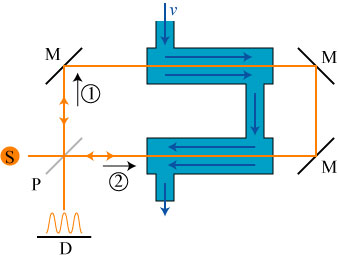
\includegraphics[width=0.38\textwidth]{Grafica/Fizeau.jpg}
    \caption{Esperimento di Fizeau}
    \label{fig:fizeau}
\end{center}
\end{wrapfigure}
Un altro esperimento, effettuato da Fizeau nel 1851, sembra confermare questa ipotesi.\\
Una sorgente di luce monocromatica illumina uno specchio semiargentato, che crea due raggi. Tramite una serie di specchi, ciascun raggio attraversa due tubi in cui scorre dell'acqua: un raggio sempre in verso concorde, e l'altro sempre in verso opposto.\\
Dopo l'attraversamento i due raggi vengono ricombinati su uno schermo, dove generano una figura di interferenza, da cui è possibile misurare la differenza dei due percorsi.\\
Se il trascinamento dell'etere fosse completo allora la velocità di ciascun raggio sarebbe $c' = c\pm v_w$, dove $v_w$ è la velocità dell'acqua. Ciò darebbe luogo a uno sfasamento significativo, che non viene però osservato.\\
L'esito è invece a favore della teoria di Fresnel\footnote{Come si vedrà nei prossimi paragrafi, la formula di Fresnel costituisce un caso particolare delle più generali leggi di composizione delle velocità di Einstein}, che prevede uno sfasamento molto minore, in quanto il trascinamento è solo parziale:
\[
c' = \frac{c}{n} \pm v_w \left ( 1-\frac{1}{n^2} \right )
\]
Tuttavia un trascinamento parziale non è compatibile con l'esperimento di Michelson-Morley: poiché l'aria non \textit{trascina} l'etere, si dovrebbe osservare una differenza di percorso tra i due raggi, che tuttavia non viene rilevata.\\
Ancora più grave è il fatto che secondo la formula di Fresnel la velocità della luce dipenderebbe dalla lunghezza d'onda usata, in quanto l'indice di rifrazione $n$ dipende da essa. Bisognerebbe allora ipotizzare un etere diverso per ciascuna delle infinite frequenze possibili della luce.\\
Tale dipendenza, comunque, non viene sperimentalmente osservata.

\subsubsection{Contrazione di Lorentz-Fitzgerald}
Nel 1892, per spiegare l'esito nullo dell'esperimento di Michelson-Morley nell'ipotesi di un etere parzialmente trascinato, Fitzgerald ipotizzò che, poiché i campi elettromagnetici sono alterati in un sistema di riferimento in moto (come era stato derivato qualche anno prima da Heaviside tramite le equazioni di Maxwell), potrebbero esserlo anche le forze intermolecolari che definiscono le dimensioni macroscopiche di un oggetto solido. Un oggetto in moto, perciò, potrebbe \textit{contrarsi} nella direzione del moto di un fattore $\sqrt{1-v^2/c^2}$.\\
Nell'esperimento di Michelson-Morley, perciò, se $L_1$ è la lunghezza del braccio nella direzione del moto durante il moto, e $L_1^0$ quella che avrebbe in quiete, si avrà che $L_1 = L_1^0 * \sqrt{1-v^2/c^2}$. Sostituendo nelle relazioni ricavate precedentemente:
\[
T_{dir.} = \frac{2L_1}{c\left (1-\frac{v^2}{c^2}\right )} = \frac{2L_1^0 \sqrt{ 1-\frac{v^2}{c^2}}}{c\left (1-\frac{v^2}{c^2}\right )} = \frac{2L_1^0}{c\sqrt{1-\frac{v^2}{c^2}}} = T_{trasv.} \Rightarrow \Delta t = 0 \Rightarrow \Delta t'-\Delta t = 0
\]
come misurato.\\
In ogni caso, poiché la velocità orbitale terrestre $v$ cambia a seconda del periodo dell'anno, si può misurare un $\Delta t$ in un momento e un $\Delta t''$ dopo alcuni mesi, ed esaminare eventuali variazioni, dovute al fatto che la contrazione sarà diversa. Di nuovo non si trova alcun risultato: persino l'ipotesi di contrazione delle lunghezze (considerata ad hoc ai tempi) non è in grado di salvare l'etere.

\subsection{Trascinamento dell'etere: riepilogo}
Riepilogando, vi sono tre possibilità per l'etere:
\begin{enumerate}
    \item Etere completamente stazionario: spiega l'aberrazione stellare, ma non è compatibile con gli esperimenti di Michelson-Morley, Airy o Fizeau.
    \item Etere completamente trascinato: compatibile con Michelson-Morley, ma non con Airy o Fizeau. Secondo questa ipotesi, inoltre, non dovrebbe esserci l'aberrazione stellare, che invece si osserva.
    \item Etere parzialmente trascinato: compatibile con l'aberrazione stellare e gli esperimenti di Airy e Fizeau, ma non con quello di Michelson-Morley (di precisione molto maggiore). Inoltre secondo tale ipotesi la velocità dell'etere dipenderebbe dalla frequenza della luce utilizzata, cosa che è assurda e non verificata.
\end{enumerate}
Non è quindi possibile in generale costruire un concetto di \textbf{etere} che sia compatibile con l'evidenza sperimentale. Perciò l'eventualità (a) che le leggi della meccanica definiscano un sistema di riferimento "speciale" deve essere scartata, in quanto inconsistente con le osservazioni.

\subsection{Teorie emissive: il paradosso di De Sitter}
La \textbf{teoria emissiva} propone che la luce si muova a velocità $c$ solo rispetto al sistema di riferimento della sorgente che l'ha emessa. In tal modo si rispetta il principio di relatività, e si mantengono le trasformazioni di Galileo senza modifiche.\\
Tale ipotesi spiega l'esito nullo dell'esperimento di Michelson-Morley, in quanto la sorgente è solidale all'apparato sperimentale, e perciò non c'è alcuna differenza nelle velocità dei due raggi trasversi.\\
Tuttavia ciò produce forti conseguenze a livello astronomico. Se si considera un sistema di stelle doppie (una coppia di stelle che orbita attorno al comune centro di massa) i raggi emessi a diversi periodi dell'orbita avranno velocità diverse per un osservatore a Terra. In particolare, per certe precise configurazioni (orientazione del sistema stellare, distanza, velocità di rivoluzione) alcuni raggi più veloci possono "superare" i raggi più lenti emessi precedentemente. Un osservatore vedrebbe perciò un moto "sfasato", come se dei fotogrammi fossero scambiati all'interno di un video, che non sarebbe compatibile con le leggi di Keplero. Un'animazione esplicativa del fenomeno è disponibile qui: \url{https://goo.gl/PKpFNC}.\\
Tale effetto, proposto da de Sitter, non è mai stato osservato su un campione statisticamente rilevante di sistemi binari, e perciò mina la validità di teorie simili.\\
Ciò significa che anche l'opzione (b), ossia la modifica relativistica delle equazioni di Maxwell, non è compatibile con l'evidenza sperimentale.

\section{L'origine della relatività speciale}
Come osservato nella sezione precedente, molteplici risultati sperimentali puntano sulla costanza della velocità della luce, indipendentemente dal sistema di riferimento. Non resta quindi che sostituire il postulato sull'assolutezza del tempo (per cui non può esistere una velocità limite) e sostituirlo con la costanza di $c$ in tutti i sdr.\\

\subsection{Postulati della relatività speciale}
Osserviamo che la costanza della velocità della luce in ogni sistema di riferimento inerziale è incompatibile con il postulato dell'assolutezza del tempo da cui si è partiti per ricavare le trasformazioni di Galileo.\\
Infatti, la misura del tempo dipende dalla possibilità di stabilire la simultaneità tra due eventi - quello che si osserva (es. l'arrivo di un treno) e la lettura di uno strumento opportuno (es. la lancetta di un orologio). In un universo in cui la velocità della luce è costante in tutti i sistemi di riferimento inerziali la simultaneità di due eventi dipende dal sistema di riferimento.\\
Si consideri un osservatore $C$ posto esattamente a metà di un vagone, in moto rispetto ad un osservatore $C'$ in piedi sulla banchina. Nel sistema di riferimento di $C'$, all'istante in cui $C$ passa esattamente davanti a $C'$ due fulmini colpiscono gli estremi del vagone, e $C'$ osserva gli eventi simultaneamente.\\
Tuttavia $C$ si sta muovendo in avanti, e poiché la velocità della luce è $c$ anche per lui, il segnale dal retro del vagone impiegherà un po' più di tempo a giungere a lui rispetto a quello della parte frontale. Per $C$, perciò, i due eventi non sono simultanei: il fulmine frontale cade prima.\\
È quindi necessario sostituire al postulato sull'assolutezza del tempo quello sulla costanza della velocità della luce, che è giustificato da numerosi esperimenti.\\
I postulati della relatività speciale sono quindi:
\begin{enumerate}
    \item \textbf{Omogeneità} dello spazio e del tempo, \textbf{isotropia} dello spazio.
    \item \textbf{Principio di relatività}
    \item La velocità della luce nel vuoto è la \textbf{stessa} in tutti i sistemi di riferimento inerziali. 
\end{enumerate}

\subsection{Misure di tempo e di spazio}
Rimuovendo l'assolutezza del tempo è necessario ridefinire la modalità con cui si determinano tempi e distanze.\\
Poniamoci in un sistema di riferimento inerziale, che dotiamo di orologi posti in tutti i suoi punti, \textbf{sincronizzati} tra loro. Il tempo a cui avviene un evento in tale sistema di riferimento è definito perciò da una lettura \textit{simultanea} ad esso effettuata sull'orologio la cui posizione spaziale coincide con l'evento stesso.\\
Per sincronizzare gli orologi si possono usare segnali luminosi. Per esempio, siano dati due orologi, $A$ e $B$, posti ad una certa distanza tra loro.\\
Ipotizziamo che la luce impieghi lo stesso tempo ad andare da $A$ e $B$ che impiega a tornare da $B$ a $A$\footnote{In effetti quest'ipotesi \textit{definisce} operativamente il concetto di tempo}. Da $A$ inviamo quindi un segnale luminoso a $t=0$ (misurato in $A)$ verso $B$, contro uno specchio che lo rimanda subito indietro ad $A$, che lo riceve ad un tempo $\Delta t$. Appena $A$ riceve il segnale legge il tempo di $B$. Se quest'ultimo tempo è pari a $\Delta t/2$ allora gli orologi in $A$ e $B$ sono sincronizzati: questo perché il ritorno dell'impulso luminoso dallo specchio coincide con l'arrivo del segnale luminoso che indica la posizione delle lancette di $B$ all'istante della riflessione, che corrisponde al tempo della sola andata - e quindi deve essere metà del tempo necessario all'andata e al ritorno.\\

Una volta definite le misure temporali, possiamo misurare le distanze tra due punti (o la lunghezza di un segmento) effettuando una misura di posizione \textbf{allo stesso tempo}.

Notiamo che le misure di tempi e lunghezze, poiché si originano dal concetto di simultaneità, sono \textbf{relative} al sistema di riferimento in cui sono effettuate. Un altro sistema di riferimento non concorda sulla sincronizzazione degli orologi, e quindi non concorda sulla misura di tempi e lunghezze.

\subsection{Trasformazioni di Lorentz}
Ci proponiamo ora di ricavare le relazioni matematiche che collegano tempi e posizioni misurati in sistemi di riferimento inerziali \textbf{differenti}.\\
Consideriamo due sistemi di riferimento inerziali $S$ e $S'$, con $S'$ in moto a velocità $\vec{v}$ rispetto a $S$.\\
Tutte le considerazioni su omogeneità dello spazio e del tempo e isotropia dello spazio sono mantenute dal caso delle trasformazioni di Galileo. Mantenendo inoltre le stesse semplificazioni di calcolo (assi paralleli tra i due sdr, origini coincidenti per $t=0$, moto esclusivamente lungo l'asse $\hat{x}$) possiamo partire da:
\[
x' = ax - bt \Leftrightarrow x = ax'+bt'
\]
con $b/a = v$, ossia la velocità relativa tra i due sdr inerziali (a seguito degli stessi ragionamenti fatti nel caso galileiano).\\
Imponiamo quindi la costanza della velocità della luce $c$, per cui $x = ct \Rightarrow x' = ct'$. Sostituendo nelle trasformazioni:
\[
ct' = x' = a(ct) - bt = (ac - b)t \Leftrightarrow ct = x = a(ct') + bt = (ac+b)t' 
\]
Dalla prima si ottiene:
\[
t' = \frac{ac-b}{c}t
\]
Che sostituita nella seconda conduce a:
\[
c\cancel{t} = (ac+b)t' = (ac+b)\frac{(ac-b)}{c}\cancel{t} \Rightarrow c^2 = a^2c^2- b^2 = a^2(c^2-v^2)
\]
Dove si è usata la relazione $b/a = v$
Risolvendo quindi per $a$:
\[
a^2 = \frac{c^2}{\displaystyle c^2\left (1-\frac{v^2}{c^2}\right )}\Rightarrow a = \gamma(v) = \sqrt{\frac{1}{\displaystyle 1- \frac{v^2}{c^2}}}
\]
Perciò possiamo riscrivere la trasformazione:
\[
x' = ax -bt = a(x -\frac{b}{a}t) = \gamma(x-vt) \Leftrightarrow x = \hlc{Yellow}{\gamma(x'+vt')}
\]
Basta ora invertire la prima relazione per ottenere la trasformazione per il tempo:
\begin{align*}
\frac{x'}{\gamma}=x-vt \Rightarrow vt &= \hlc{Yellow}{x}-\frac{x'}{\gamma} = \gamma(x'+vt')-\frac{x'}{\gamma} = \gamma x' - \frac{x'}{\gamma} + \gamma vt' = \\
&= x'\gamma\left (\hlc{SkyBlue}{1-\frac{1}{\gamma^2}} \right ) + \gamma v t'
= x'\gamma\left (\hlc{SkyBlue}{\frac{v^{\cancel{2}}}{c^2}} \right ) + \gamma \cancel{v} t' = \cancel{v}t\\
&\Rightarrow t = \gamma\left ( x'\frac{v}{c^2}+t' \right ) \Leftrightarrow t' = \gamma\left ( t - \frac{v}{c^2}x \right )
\end{align*}
Per quanto riguarda gli altri assi è possibile ripetere le stesse considerazioni (che derivano dal principio di relatività stesso) effettuate nel caso galileiano. Perciò le trasformazioni di Lorentz (a meno delle semplificazioni dei conti) sono date da:
\[
\begin{cases}
x' = \gamma(x-vt)\\
y' = y\\
z' = z\\
t' = \gamma\left ( t-\frac{v}{c^2}x \right )
\end{cases} \Leftrightarrow 
\begin{cases}
x = \gamma(x'+vt')\\
y = y'\\
z = z'\\
t = \gamma\left ( t' + \frac{v}{c^2}x' \right )
\end{cases}
\]
(Qui vale sempre la convenzione per cui il sdr con l'apice è quello in \textit{moto} rispetto al primo, considerato "in \textit{quiete}". $v$ è positiva se il sdr che si sposta si sta allontanando, mentre è negativa se si sta avvicinando.) 

Osserviamo che per $v \ll c$ (o, equivalentemente, per $c\to +\infty$), $\gamma = 1/\sqrt{1-\beta^2} \to 1$, e le trasformazioni di Lorentz si riconducono a quelle galileiane. Gli effetti relativistici compaiono solo quando le velocità in gioco divengono frazioni significative di $c$.

\section{Conseguenze della relatività}
Esaminiamo ora le conseguenze fisiche delle trasformazioni di Lorentz.

\subsection{Simultaneità}
La relatività della simultaneità compare immediatamente dall'uso delle trasformazioni di Lorentz.\\
Si considerino due eventi $A$ e $B$. Rispetto ad un primo sistema di riferimento $S$ si determinano posizione e istante in cui avvengono, ottenendo $(x_A, y_A, z_A, t_A)$ e $(x_B, y_B, z_B, t_B)$. L'intervallo di tempo è tra di essi è quindi $\Delta t = t_B-t_A$, e i due eventi sono simultanei in $S$ se $\Delta t = 0$.\\
Rispetto ad un secondo sistema di riferimento $S'$, in moto a velocità $v$ rispetto a $S$ lungo il suo asse $x$, le stesse misurazioni restituiscono, secondo le trasformazioni di Lorentz:
\[
t_B' = \gamma\left (t_B - \frac{v}{c^2}x_B \right ); \quad t_A' = \gamma \left ( t_A - \frac{v}{c^2}x_A \right ) 
\]
In $S'$ l'intervallo di tempo tra i due eventi è quindi:
\[
\Delta t' = t_B' - t_A' = \gamma\left ( \Delta t - \frac{v}{c^2}\Delta x \right ); \quad \Delta x = x_B - x_A
\]
Se i due eventi sono simultanei per $S$, non è quindi detto che lo siano per $S'$, in quanto $\Delta t' = -\gamma v/c^2 \Delta x \neq 0$.\\
Se tuttavia due eventi avvengono simultaneamente nello stesso punto dello spazio per un osservatore, allora saranno simultanei (e coincidenti) rispetto a tutti i sistemi di riferimento, come si può notare ponendo $\Delta x = 0$ nella relazione appena trovata.\\

D'altro canto, un segnale luminoso appare allo stesso modo rispetto a tutti i sistemi di riferimento, in quanto la sua velocità è sempre $c$. Verifichiamolo.\\
Consideriamo una sorgente puntiforme all'origine di un sistema di riferimento inerziale $S$, che emette un segnale in tutte le direzioni a $t=0$. Ad un generico istante $t$, il segnale avrà la forma di una "sfera di luce" di raggio $ct$, data da:
\[
x^2 + y^2 + z^2 = ct^2
\]
Un osservatore $S'$ è in moto a velocità $v$ lungo $x$ rispetto a $S$. Consideriamo il caso di sistemi di riferimento con assi allineati, le cui origini coincidono al momento di emissione del segnale. Dall'applicazione delle trasformazioni di Lorentz si ottiene:
\begin{align*}
&\gamma^2(x' + vt')^2 + y'^2 + x'^2 = c^2 \gamma^2 \left ( t' + \frac{v}{c^2}x' \right )^2\\
&\Rightarrow \gamma^2 (x'^2 + v^2t'^2 + \bcancel{2vx't'}) + y'^2 + z'^2 = \gamma^2 \left ( c^2 t'^2 + \frac{v^2 x'^2}{c^2} + \bcancel{2vx't'} \right )\\
&\Rightarrow \gamma^2 x'^2 \left (1 -\frac{v^2}{c^2} \right ) + y'^2 + z'^2 = \gamma^2 c^2 t'^2 \left ( 1-\frac{v}{c^2}\right ) \Rightarrow x'^2 + y'^2 + z'^2 = c^2 = c^2 t'^2
\end{align*}
Anche l'osservatore in $S'$ osserva una "sfera di luce" con centro l'origine del suo sdr espandersi a partire dal tempo $t' = 0$.

\subsection{Causalità}
Se la simultaneità di due eventi è relativa, è possibile che se in un sdr $S$ l'evento $A$ causa l'evento $B$ rispetto ad un altro sdr $S'$ l'effetto preceda la causa?\\
Prima di tutto, perché $A$ possa causare $B$ tra i due deve avvenire uno scambio di informazione, che possiamo modellizzare come l'invio di un segnale da $A$ a $B$ ad una velocità $u$ rispetto a $S$. In $S$ si avrà perciò:
\[
x_B- x_A = u(t_B -t_A); \quad \Delta t = t_B-t_A > 0
\]
Un generico sistema di riferimento $S'$ in moto lungo $x$ a velocità $v$ rispetto a $S$ osserverà:
\[
\Delta t' = \gamma \left [(t_B-t_A) - \frac{v}{c^2} (x_B-x_A) \right ] = \gamma \left [ \Delta t - \frac{v}{c^2} u\Delta t \right ] = \gamma \Delta t \left [ 1-\frac{vu}{c^2}\right ]
\]
$\gamma > 1$ in ogni caso, e se $v$ e $u$ sono entrambi $< c$, il termine tra parentesi non può essere negativo, quindi si avrà $\Delta t' > 0$, ossia anche l'osservatore in $S'$ vede avvenire prima la causa $A$ e poi l'effetto $B$.\\
Perché quindi la relatività possa essere consistente con le osservazioni è necessario ipotizzare che nulla possa muoversi a velocità maggiore di $c$\footnote{In effetti, dalla dinamica si può dimostrare che per accelerare un corpo stazionario a $c$ è necessaria energia infinita, ma nulla vieta l'esistenza di oggetti che viaggiano \textit{fin dall'inizio} a velocità $>c$, per esempio i \textbf{tachioni}. Si tratta ovviamente solo di ipotesi, e sperimentalmente si osserva che ogni particella si muove al massimo a $c$.}

\subsection{Intervallo spazio-temporale}
Si definisce \textbf{intervallo spaziotemporale} la grandezza $\Delta s$ data da:
\[
\Delta s^2 = c^2 t^2 - x^2
\]
Si dimostra che ogni osservatore misura lo stesso intervallo spaziotemporale. Per esempio, sia $S'$ in moto lungo $x$ a velocità $v$ rispetto a $S$. Per trasformazioni di Lorentz:
\[
\Delta s^2 = c^2 \left ( t' + \frac{v}{c^2}x' \right )^2 \gamma^2 %[TO DO] Finire
\]

\subsection{Contrazione delle lunghezze}
Siano $S$ e $S'$ due sistemi di riferimento inerziali in moto l'uno rispetto all'altro con una velocità $v$ diretta lungo l'asse $\hat{x}$. Consideriamo un'asta \textit{rigida} a riposo in $S$, allineata lungo l'asse $\hat{x}$. Si definisce \textbf{lunghezza} la distanza tra le sue due estremità $x_1$ e $x_2$, misurate allo stesso istante $\bar{t}$. Se la misura avviene rispetto al sdr in cui l'asta è in quiete allora otterremo la cosiddetta \textbf{lunghezza propria} $L_0$:
\[
L_0 = |x_2(\bar{t})-x_1(\bar{t})|
\]
Per determinare la lunghezza dell'asta rispetto all'altro sistema di riferimento $S'$ applichiamo le trasformazioni di Lorentz:
\[
x_1' = \gamma(x_1-v\bar{t}); \quad x_2' = \gamma(x_2 - v\bar{t})
\]
da cui si ricava:
\[ %SISTEMARE
L' = x_2'-x_1' = \gamma(
\]

\subsection{Dilatazione dei tempi} %Orologio a luce

\subsubsection{Vita media dei muoni}

\subsection{Effetto doppler} %Suoni vs luce

\subsection{Trasformazioni delle velocità}

\subsubsection{Esperimento di Fizeau}

\subsubsection{Aberrazione stellare}



\section{Paradossi della relatività}

\subsection{Paradosso dei gemelli}

\subsection{Paradosso della scala} %o del pattinatore


\end{document}